 \documentclass[12pt]{article}
\usepackage{amsmath}
\usepackage{graphicx}
\usepackage{enumerate}
\usepackage{natbib}
\usepackage{url} % not crucial - just used below for the URL 

%\pdfminorversion=4
% NOTE: To produce blinded version, replace "0" with "1" below.
\newcommand{\blind}{0}
\newcommand*{\KeepStyleUnderBrace}[1]{%f
\mathop{%
\mathchoice
{\underbrace{\displaystyle#1}}%
{\underbrace{\textstyle#1}}%
{\underbrace{\scriptstyle#1}}%
{\underbrace{\scriptscriptstyle#1}}%
}\limits
}
\usepackage{mathtools}
\mathtoolsset{showonlyrefs}
\usepackage{amsmath,amssymb,amsthm,bm,hyperref,enumerate}
\usepackage{dsfont,listings}

\usepackage[ruled,vlined]{algorithm2e}

\usepackage{enumitem}
\newtheorem{schm}{Scheme}
\newtheorem*{schm*}{Scheme}
\newtheorem{thm}{Theorem}[section]
\newtheorem{lem}{Lemma}
\newtheorem{prop}{Proposition}
\newtheorem{pro}{Property}
\newtheorem{assumption}{Assumption}
\newtheorem{cor}{Corollary}[section]
\newtheorem{defn}{Definition}
\newtheorem{example}{Example}
\newtheorem{rmk}{Remark}
\newtheorem{clm}{Claim}
% DON'T change margins - should be 1 inch all around.
\addtolength{\oddsidemargin}{-.5in}%
\addtolength{\evensidemargin}{-.5in}%
\addtolength{\textwidth}{1in}%
\addtolength{\textheight}{-.3in}%
\addtolength{\topmargin}{-.8in}%
\usepackage{xcolor}

\input macros.tex
\begin{document}
\setcounter{secnumdepth}{3}
%\bibliographystyle{natbib}

\def\spacingset#1{\renewcommand{\baselinestretch}%
{#1}\small\normalsize} \spacingset{1}
\def\fixme#1#2{\textbf{\color{red}[FIXME (#1): #2]}}




%%%%%%%%%%%%%%%%%%%%%%%%%%%%%%%%%%%%%%%%%%%%%%%%%%%%%%%%%%%%%%%%%%%%%%%%%%%%%%

\if1\blind
{
  \title{\bf Model free probability estimation for matrix feature}
  \author{Author 1\thanks{
    The authors gratefully acknowledge \textit{please remember to list all relevant funding sources in the unblinded version}}\hspace{.2cm}\\
    Department of YYY, University of XXX\\
    and \\
    Author 2 \\
    Department of ZZZ, University of WWW}
  \maketitle
} \fi

\if0\blind
{
  \bigskip
  \bigskip
  \bigskip
  \begin{center}
    {\LARGE\bf Nonparametric learning with matrix-valued predictors in high dimensions}
\end{center}
  \medskip
} \fi

\bigskip
\begin{abstract}
We consider the problem of learning the relationship between a binary label response and a high-dimensional matrix-valued predictor. Such data problems arise commonly in brain imaging studies, sensor network localization, and personalized medicine. Existing regression analysis often takes a parametric procedure by imposing a pre-specified relationship between variables. However, parametric models are insufficient in capturing complex regression surfaces defined over high-dimensional matrix space. Here, we propose a flexible nonparametric framework for various learning tasks, including classification, level set estimation, and regression, that specifically accounts for the matrix structure in the predictors. Unlike classical approaches, our method adapts to the possibly non-smooth, non-linear pattern in the regression function of interest. The proposal achieves prediction and interpretability simultaneously via a joint optimization of prediction rules and dimension reduction in the matrix space. Generalization bounds, estimation consistency, and convergence rate are established. We demonstrate the advantage of our method over previous approaches through simulations and applications to  {\color{red}XXX} data analyses. 
\end{abstract}

\noindent%
{\it Keywords:} Nonparametric learning, matrix-valued predictors, high dimension, classification, level-set estimation, regression.
\vfill


\newpage
\spacingset{1.5} % DON'T change the spacing!
\section{Introduction}
\label{sec:intro}


\section{Introduction (skipped)}
Consider a statistical learning setting where we would like to model the relationship between a matrix-valued predictor $\mX \in \mathbb{R}^{d\times d}$ and a binary label response $Y\in\{-1,1\}$. Matrix-valued predictors ubiquitously arise in modern applications. One example is from electroencephalography studies of alcoholism. The data set records voltage value measured from 64 channels of electrodes on 256 subjects for 256 time points~\citep{zhou2014regularized}. Each feature is a $256\times 64$ matrix and the response is a binary indicator of subject being alcoholic or control. Another example is pedestrian detection from image data. Each image is divided into 9 regions where local orientation statistics are generated with a total of 22 numbers per region. This yields a $22 \times 9$ matrix feature and a binary label response indicating whether the image is pedestrian~\citep{Shashua2004Pedestrian}. 


Our motivating problem for learning with matrix-valued predictors comes from brain network analysis. Label prediction based on networks is an important problem in neuroscience. In these studies, each individual in the sample is represented by their own brain network, and the nodes (brain regions of interest) shared across all networks are mapped onto a common atlas. In our analysis of human connectom project, 68 brain nodes are extracted from six functional brain regions. A connectivity is computed for every pair of nodes, resulting in an adjacency matrix of size 68 $\times$ 68 for each individual (see Figure 1). The main scientific goal is to predict the individual's disease status based on the brain connectivity network. Two main approaches have been used in the existing literature. One approach is to reduce the network to its global summary measures such as the average degree, clustering coefficient, or average path length, and use those measures as features for disease predicting. An alternative approach to label predicting is to treat connectivity network as a ``bag of non-ordered edges,'' which essentially vectorized the adjacency matrix and ignoring the network nature of the predictor. This approach suffers from ....The number of individual ..., much smaller than the predictor dimension... 

In the above examples and many other studies, researchers are interested in {\it interpretable prediction}, where the goal is to not only make accurate prediction but also identify features that are informative to the prediction. While classical learning algorithms have been successful in prediction with vector-valued predictors, the key challenge with matrix-valued predictors is the high-dimensional, complex structure in the feature space. A naive approach is to transform the feature matrices to vectors and apply classical methods based on vectors to solve the problem. However, this vectorization would destroy the structural information of the data matrices. Moreover, the reshaping matrices to vectors results in high dimensionality which leads to overfitting. 
Notably, the ambient dimension with matrix feature, $d_1d_2$, is often comparable to, or even exponentially larger than the number of sample, $n$. 
%Modern applications are often in the high dimensional regime where $d_1d_2$ is comparable to, or even larger, than the sample size $n$. 
{\color{red} feature selection...}
Our method exploits the structural information in the data matrix to overcome these challenges. 

Our goal in this paper is to develop a distribution-free prediction method that respects the matrix structure of the predictors and produces more interpretable results. We use structured sparsity penalties to incorporate the network information by penalizing both the number of simple modules and the number of nodes selected.... 

The classification problem has long been interested. Many attempts have been developed and performed well for example, decision tree, nearest neighbor, neural network and support vector machine to name a few. However, most of methods have focused on vector valued features. In many classification problems, the input features are naturally represented as matrices or tensors rather than vectors. 


Knowledge about the class probability itself is of significant interest and can tell us the confidence of the outcome of classification. Traditionally, the regression problem is addressed through distribution assumption like logistic regression or linear discriminant analysis (LDA). In many applications, however, it is often difficult to  justify the assumptions made in logistic regression or satisfy the Gaussian assumption in LDA. These issues become more challenging for matrix features because of high dimensionality.
We establish distribution free method for estimating the regression function based on level set estimation. 

Other examples can be found in medical decision making. In Osteosarcoma treatment, the degree of tumor necrosis is used to guide the choice of postoperative chemotherapy \citep{man2005expression}. Patients with $\geq 90 \%$ necrosis is labeled as 1, which is response variable $y$. Suppose that $\mX$ is a feature matrix collected from the patient such as gene expression levels on each tissue. Knowledge of the regression level set is needed to allow effective postoperative chemotherapy without a biopsy. 
We consider a nonparametric way to estimator the $\pi$-level set of the regression function based on classification problem.


Notation: For a given set $A\subset \mathbb{R}^{d_1\times d_2}$, we use $\mathds{1}\{A\}\in\{0,1\}$ to denote the indicator function, and $I(A) =\{-1,1\}$ to denote the (shifted) indicator function. A set $A$ uniquely defines an indicator function $I(\mX\in A)$ from $\mathbb{R}^{d_1\times d_2}\to \{-1,1\}$. We also use $\sign(f)\in\{-1,1\}$ to denote the sign of function $f$; that is, $\sign f=1$ if $f>0$ and $\sign f=-1$ if $f\leq 0$. We restrict to Borel-measurable functions {\color{red}{and} L2}? Do we require $\{\mX:p(\mX)=1/2\}$ to have measure zero??  %The probabilistic notions, $\mathbb{P}, \mathbb{E}, \text{Var}$, are taken with respect to both predictor and response, or with respect to predictor only. 
We use $\mathcal{MN}(\mB, \mSigma_1, \mSigma_2)$ to denote the matrix normal distribution, meaning $\text{vec}(\mX)\sim\mathcal{N}(\text{vec}(\mB), \mSigma_1\otimes \mSigma_1)$. Given a $d_1$-by-$d_2$ matrix $\mB$, we use $\mB_i$ to denote the $i$-th row of $\mB$, where $i\in[d_1]$. We use $\newnormSize{}{\cdot}_p$ to denote the $p$-norm for vectors for $p\geq 0$. The $(p,q)$-norm of a matrix $\mB$ is defined as $\newnormSize{}{\mB}_{p,q}=\newnormSize{}{\mb}_q$, where $\mb=(\newnormSize{}{\mB_1}_p,\ldots,\newnormSize{}{\mB_{d_1}}_p)\in\mathbb{R}^{d_1}$ consists of the $p$-norms for each of the rows in $\mB$. In particular, $\newnormSize{}{\mB}_{1,0}=\#\{i\in [d_1]\colon \mB_i\neq 0\}$ denotes the number of non-zero rows in $\mB$, and $\newnormSize{}{\mB^T}_{1,0}$ denotes the number of non-zero columns in $\mB$.

Need consistent notation $\mathbb{P}$, $\mathbb{P}_{\mX,y}$, $\mathbb{P}_{\mX}$. 


\section{Three learning problems}
In this section we present the main learning goals of our interest. Let $\mX\in\mathbb{R}^{d_1\times d_2}$ denote the matrix-valued predictor, $y\in\{0,1\}$ denote the binary label response, and $\mathbb{P}_{\mX,Y}$ denote the unknown joint probability distribution over the pair $(\mX,y)$. Suppose that we observe a sample of $n$ training data points, $(\mX_1,y_1),\ldots,(\mX_n,y_n)$, identically and independently distributed (i.i.d.) according to $\mathbb{P}_{\mX,y}$. Let $(\mX_{n+1},y_{n+1})$ be a new test point drawn independently from the same distribution. Our goal is to make reliable prediction about $y_{n+1}$ given the new feature value $\mX_{n+1}$, with no strong distributional assumptions other than i.i.d.\ data. When no confusion arises, we often omit the subscript $(n+1)$ and simply write $(\mX,y)$ for the prototypical test point. 
%The problem of learning is to find a decision function $f\colon \mathbb{R}^{d_1\times d_2}\to \mathbb{R}$ that minimizes certain expected risk $R(f)$ under the unknown distribution $\mathbb{P}_{\mX,y}$. The expected risk $R(f)$ is a functional over a given class of candidate functions $f\in\tF$; the form of risk depends on the specific learning goals which are detailed in the next paragraph. 

We consider three main supervised learning problems: classification, level set estimation, and regression. 

\begin{enumerate}[label={2.\arabic*},wide, labelwidth=!, labelindent=0pt]
\item {\it Classification}: Classification is the problem of predicting the label $y\in \{-1,1\}$ to which a new matrix observation $\mX$ belongs. A prediction rule (also called a classifier) decides that $y=1$ if $\mX\in S$ and $y=0$ if $\mX \not\in S$, where $S$ is a Borel subset of $\mathbb{R}^{d_1\times d_2}$. The set $S$ uniquely defines an indicator function, $I(\mX\in S)$, in the matrix space. With a little abuse of notations, we will use the term ``classifier'' to refer to as both the set $S$ and its associated indicator function $I(\mX\in S)$.
%and write $S\in \tS$ to denote the classifier form a given candidate set. 
We formulate the classification problem as choosing a classifier that minimizes the expected classification error,
\begin{equation}\label{eq:classloss}
%R(f) = \mathbb{P}_{\mX,y}\left(y\neq \sign f(\mX)\right), 
R(S)=\mathbb{P}\left[y\neq I(\mX\in S)\right], \quad \text{for all}\ S\in\tS,
\end{equation}
where $\tS$ is a given set of candidate classifiers, and the probability is taken over the pair $(\mX,y)$ according to the joint distribution $\mathbb{P}_{\mX,y}$.
The expected classification error $R(S)$ is also referred to as the classification risk. %The expected classification error $R(S)$ describes the probability when the true label and predicted label differs. 
%Note that we have used $\sign f$ to denote the binary-valued classifier, in order to distinguish from the real-valued decision function $f$. In general, it is common, but not necessary, to estimate $\sign f$ through $f$. 
When the candidate set $\tS$ consists of all Borel subsets of $\mathbb{R}^{d_1\times d_2}$, the minimizer of~\eqref{eq:classloss} is called the Bayes classifier. It is known that (one of) the Bayes classifier can be written as 
\begin{equation}\label{eq:bayes}
%\bayesf (\mX)=\sign\{ p(\mX)- 1/2\}.
\bayesS\{\mX\in\mathbb{R}^{d_1\times d_2}\colon p(\mX)\geq 1/2\},
\end{equation}
where $p(\mX)=\mathbb{P}(y=1|\mX)$ is the conditional probability function defined in matrix space. In principle, Bayes classifier is non-unique because of the arbitrary prediction rules allowed on the boundaries $\partial S_{\text{bayes}} = \{\mX\colon p(\mX)=1/2\}$. Without loss of generality, we will use~\eqref{eq:bayes} as the canonical form of Bayes classifier. 

In practice the population joint distribution $\mathbb{P}_{\mX,y}$ is unknown, so the objective function~\eqref{eq:classloss} and the minimizer~\eqref{eq:bayes} need to be estimated through the data $(\mX_i,y_i)_{i=1}^n$. The first goal of our paper is to estimate the Bayes classifier for matrix classification:

{\bf Question 1.} When matrix dimension $d_1d_2$ far exceeds the sample size $n$, how to efficiently perform matrix classification without much assumptions on $\mathbb{P}_{\mX,y}$?



\item {\it Level set estimation}: The problem of level set estimation generalizes the classification task. 
%Let $p(\mX)=\mathbb{P}(y=1|\mX)$ denote the conditional probability function over the matrix space $\mathbb{R}^{d_1\times d_2}$. 
%Note that $p(\mX)$ is a bounded function over $\mathbb{R}^{d_1\times d_2}$, because of $y$ is labeled by $\pm 1$. 
For a given $\pi\in[0, 1]$, the $\pi$-level set of the conditional probability function $p(\mX)$ is defined by
\begin{equation}\label{eq:level}
\bayesS(\pi) = \{\mX\in\mathbb{R}^{d_1\times d_2}\colon p(\mX)\geq \pi\}.
\end{equation}
%The set $S(\pi)$ uniquely defines an indicator function, $\mathds{1}\{\mX\in S(\pi)\}$, over the matrix space. 
An important characterization of $\pi$-level set is that it is the optimal weighted classifier~\citep{willett2007minimax,scott2007regression,wang2008probability}. Specifically, among all Borel subsets of $\mathbb{R}^{d_1\times d_2}$, $S_{\text{bayes}}(\pi)$ minimizes the expected $\pi$-weighted classification error,
\begin{equation}\label{eq:risklevel}
%R(f)=\mathbb{E}_{\mX,y}\left[w(y)I\left(y\neq \sign f(\mX)\right) \right],
R_\pi(S)=\mathbb{E}\left[ w_{\pi}(y)\mathds{1}(y\neq I(\mX\in S))\right],
\end{equation}
where the expectation is taken jointly over $(\mX,y)$, and we define $w_{\pi}(y)=1-\pi$ if $y=1$ and $w_{\pi}(y)=\pi$ if $y=-1$; that is, $w_{\pi}(\cdot)$ assigns possibly unequal weights for the two labels. In light of~\eqref{eq:classloss} and~\eqref{eq:risklevel}, the level set estimation problem is an extension to $\pi$-weighted classification of the usual classification with $\pi=1/2$. In particular, the $\pi$-level set $S_{\text{bayes}}(\pi)$ serves the role of Bayes classifier in the risk minimization. Accurate level set estimation plays an important role in applications of geographical elevation maps, imaging contour detection, and motion tracking. We consider the following question in our context:

{\bf Question 2.} How to simultaneously estimate the level set and identify important variables in the matrix-valued predictors $\mX$, for the goal of interpretable prediction?


\item {\it Nonparametric regression}: The problem of nonparametric regression is to estimate the conditional mean $\mathbb{E}(y|\mX)$ as a continuous-valued function defined in the matrix space. In the context of binary response with $\{-1,1\}$ labels, estimating regression is equivalent to estimating conditional probability $p(\mX)=\mathbb{P}(y=1|\mX)=2\mathbb{E}(y|\mX)-1$. Throughout the paper we will work with $p(\mX)$ and refer to it as the regression function. The function $p(\mX)$, among all measurable functions $f\colon \mathbb{R}^{d_1\times d_2}\to[0,1]$, minimizes the expected squared error (also known as regression risk),
\begin{equation}\label{eq:regression}
R_{\text{reg}}(f)=\mathbb{E}\left[y+1-2f(\mX)\right]^2,
\end{equation}
where the expectation is taken jointly over $(\mX,y)$. Our final goal is the function estimation:

{\bf Question 3.} How to achieve accurate and interpretable learning of the regression $p(\mX)$ as a function in the high-dimensional matrix space $\mathbb{R}^{d_1\times d_2}$?
\end{enumerate}


Matrix-valued predictors impose unique challenges to the aforementioned three problems. We consider nonparametric learning without imposing particular function forms of $\mathbb{P}_{\mX,y}$, and we allow matrix dimension $d_1d_2$ to grow sub-exponentially with the sample size $n$. This scenario is important yet notably hard for three reasons. First, matrix-valued predictors represent various aspects of data features including global structure (e.g.\ clustering patterns, community hubs) and local structure (e.g.\ node degrees, edge connection). While classical learning algorithms have been successful with multivariate predictors invariant to indexing, challenge arises with structured predictors represented by matrices. Second, nonparametric methods typically rely on some notion of local smoothness in the predictor domain. Extracting useful neighborhood structure in the matrix-valued predictor domain has yet to explore. Third, matrix-based prediction often lead to high dimension low sample size problems. This setting brings challenges to interpretable prediction. Unlike parametric models, non-parametric learning makes little assumptions on the variable relationships, which adds complexity to interpretation. Achieving accurate prediction while maintaining descriptive simplicity is therefore our main goal. 

%“learning reduction” from one supervised learning problem to another which is more fundamental or better understood. Our approach finds classification rule first and address the level set estimation and regression problem in order. We blend the level set approach in functional optimization with label-sensitive classification in statistical machine learning, and take the best out of the two worlds. 




\section{From classification to regression: a new deal}\label{sec:idea}
The three problems of our interest represent a range of learning tasks with increasing difficulties. Classification is a special case of level set estimation with $\pi=1/2$, whereas the level set is a discrete approximation of the regression function. A common approach is to address regression first, and then solve the earlier two using plug-in estimators (Figure~\ref{fig:diagram}a). This procedure, however, undermines the fact that regression is generally harder than the other two. Indeed, as we show in Section~\ref{sec:theory}, regression has a slower convergence rate $\tO(n^{-1/2})$ compared to the fast rate $\tO(n^{-1})$ of classification. 
Ignorance of the increased complexity violates Vapnik’s maxim: \emph{When solving a given problem, one should try to avoid solving a more general problem as an intermediate step.} 

\begin{figure}
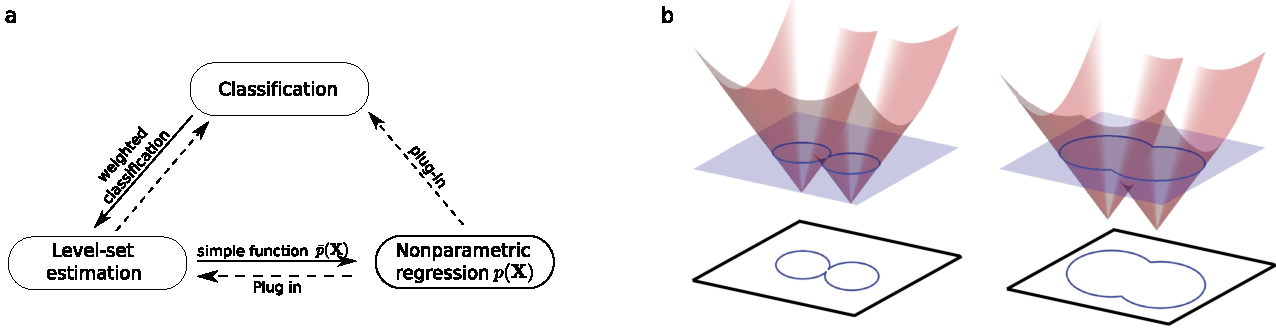
\includegraphics[width=16cm]{level.pdf}
\caption{(a) Our learning reduction approach (solid line) to three learning problems and classical plug-in approaches (dashed line). (b) Schematic diagram for nonparametric function estimation via level set estimation (Figure modified from~\cite{gibou2018review}).}\label{fig:diagram}
\end{figure}

Following Vapnik's principle, we develop a ``learning reduction'' approach by relating the regression problems to classifications, which are more fundamental and easier to address. In this section we restrict our attention to the population properties of regression function $p(\mX)$ when the true distribution $\mathbb{P}_{\mX,y}$ is known. This ideal situation leads to a cleaner characterization with known (deterministic) objective functions in~\eqref{eq:classloss}, \eqref{eq:risklevel}, and \eqref{eq:regression}. The finite sample estimation will be presented in Section~\ref{sec:theory}, in which we address the general case with unknown distribution $\mathbb{P}_{\mX,y}$, and the only information is through empirical (stochastic) risk estimated from the training set $(\mX_i,y_i)_{i=1}^n$. 
%The theoretical and algorithmic benefits of our approach will be demonstrated in Sections~\ref{sec:theory}-\ref{sec:algorithm}.


\subsection{Level set approaches to nonparametric matrix regression}\label{sec:bridge}
Our building block is to use level sets to estimate regression function $p(\mX)$ through classifications. The level set approach bridges the two sides of a same coin -- characteristic (set indicator) functions in functional analysis and weighted classifications in statistical learning -- in order to take the best of the two worlds. Specifically, let $p(\mX)\colon \mathbb{R}^{d_1\times d_2}\to [0,1]$ be the target regression function of interest. Let $\Pi=\{{1/H}, {2/H}, \ldots, {(H-1)/ H} \}$ be a sequence of evenly spaced points in $[0,1]$, where $H\in\mathbb{N}_{+}$ is the smoothing parameter. We introduce an $H$-step function from $\mathbb{R}^{d_1\times d_2}$ to $[0,1]$,
\begin{equation}\label{eq:stepfunction}
\bar p(\mX)= {1\over 2H}  \sum_{\pi \in \Pi} I(\mX\in \bar S(\pi))+{1\over 2},
\end{equation}
where, for every $\pi\in\Pi$, the set $\bar S(\pi)\subset \mathbb{R}^{d_1\times d_2}$ is the classifier that minimizes the $\pi$-weighted classification risk~\eqref{eq:risklevel} $R_\pi(S)$,
\begin{equation}\label{eq:constrained}
\bar S(\pi) \stackrel{\text{def}}{=} \argmin_{S\in \tS}\mathbb{E}\left[ w_{\pi}(y)\mathds{1}(y\neq I(\mX\in S))\right],
\end{equation}
subject to the constraint $S\in\tS$, with $\tS$ being a given candidate set of classifiers. 
%Here, the set $\bar S(\pi)\subset \mathbb{R}^{d_1\times d_2}$ is defined by the optimal classifier minimizing~\eqref{eq:risklevel} subject to the constraint $S\in\tS$, where $\tS$ is a given candidate set of classifiers. 
When the set $\tS$ is rich enough, e.g., $\tS$ consists of all Borel sets, then $\bar S(\pi)$ reduces to $S_{\text{bayes}}(\pi)$ in~\eqref{eq:level}. We leave the $\tS$ in general here; the specific choice of $\tS$ will be described in Section~\ref{subsec:linear class}. 

The following assumption quantifies the identification of level sets from weighted classification.  
\begin{assumption}[Identifiability]~\label{ass:identifiability} For a given $\pi\in(0,1)$, we call a level set $\bayesS(\pi)$ is identifiable from weighted classification, if there exist constants $\alpha\in(0,1]$ and $C>0$, such that
\begin{equation}\label{eq:identity}
\mathbb{P}_{\mX}\left[ S  \Delta \bayesS(\pi)\right]\leq C \left[R_{\pi}(S)-R_{\pi}(\bayesS(\pi))\right]^{\alpha}, \quad \text{for all }S\subset \mathbb{R}^{d_1\times d_2}
\end{equation}
where $S\Delta S'=\{\mX\colon \mX\in S/S' \text{ or }S'/S\}$ denotes the set difference between $S$ and $S'$. The largest possible value of $\alpha$ in~\eqref{eq:identity} is called the noise level of weighted classification. 
\end{assumption}

The condition~\eqref{eq:identity} controls the perturbation of classifier in matrix probability space $\mathbb{P}_{\mX}$ with respect to the weighted classification risk. The identifiability implies that the set $\bayesS(\pi)$ is the unique (up to a measure-zero set in $\mathbb{P}_{\mX}$) global optimizer of the weighted classification risk. The noise level $\alpha$ generally depends on the probability mass of $\mX$ and the changing behavior of $p(\mX)$ near the boundary $\partial S_{\text{bayes}}(\pi)=\{\mX\colon p(\mX)=\pi\}$. Note that $\alpha$ is upper bounded by $1$, because we always have $R_{\pi}(S)-R_{\pi}(\bayesS(\pi))\leq \mathbb{P}_{\mX}\left[S \Delta \bayesS(\pi)\right]$. In particular, $\alpha=0$ corresponds to no identifiability. 

Our first result is to bound the regression excess risk using classification excess risk.
\begin{thm}[Nonparametric regression via weighted classifications]\label{thm:twobounds}Let $p(\mX)$ be a regression function, and $\bar p(\mX)$ be the linear combination of weighted classifiers in~\eqref{eq:stepfunction}. Suppose the level sets $\{S_{\text{bayes}}(\pi)\}_{\pi \in \Pi}$ are all identifiable with constants $\alpha\in(0,1]$ and $C\in(0,\infty)$. Then,
\begin{align}\label{eq:approximation}
R_{\textup{reg}}(\bar p) - R_{\textup{reg}}(p)\leq 8\mathbb{E}_{\mX}\left| \bar p(\mX)- p(\mX)\right|\leq {8\over H}+C\sum_{\pi\in \Pi}\left[ R_{\pi}(\bar S(\pi)) -R_{\pi}(\bayesS(\pi))\right]^{\alpha}.
\end{align}
\end{thm}
Theorem~\ref{thm:twobounds} shows the key role of $\bar p(\mX)$ in bridging regression and classification. The results suggest that the estimation of $p(\mX)$ can be reduced to estimation of $\bar p(\mX)$, or equivalently, to a sequence of weighted classifications $\{\bar S(\pi)\}_{\pi\in\Pi}$. The approximation error~\eqref{eq:approximation} consists of two terms. The first term is the discretization error due to the step function approximation to the regression function, which goes to $0$ as $H\to \infty$. The second term is the excess risk in classification optimized over $\tS$ compared to that over all Borel sets, representing the capability of the candidate classifiers $\tS$. 

Estimating $\bar p(\mX)$ as a surrogate of $p(\mX)$ provides several benefits. From a statistical perspective, $\bar p(\mX)$ is a finite combination of weighted classifiers, which are easier to solve than regression. From the perspective of functional analysis, the function $\bar p(\mX)$ provides a valid approximation to $p(\mX)$ even when $p(\mX)$ is non-smooth and oscillating. In particular, the estimation of $\bar p(\mX)$ relies less crucially on the local neighborhood of $\mX$. This feature is especially appealing for matrix-valued predictors, since the predictor space is high dimensional and often barely explored by small sample size data.  

We conclude this section with a remark on the Assumption~\ref{ass:identifiability}. We show in Appendix~\ref{sec:population} that the Assumption~\ref{ass:identifiability} is equivalent to
\begin{equation}\label{eq:mass}
\mathbb{P}_{\mX}\left(|p(\mX)-\pi|\leq t \right) \leq C't^{\alpha/(1-\alpha)}, \quad \text{ for all }t\in (0,\ t_*],
\end{equation}
for some constants $t_*>0$ and $C'=C'(t_*)>0$. The condition~\eqref{eq:mass} controls the probability mass of $\mX$ located near the level set boundary $\partial S_{\text{bayes}}(\pi)=\{\mX\colon p(\mX)=\pi \}$. The value of $\alpha$ typically depends on uncertainty near the optimal decision boundary but less crucially on the predictor dimensions. Consider a simple case when the entries of matrix $\mX$ are i.i.d.\ drawn from $\text{Uniform}[-1,1]$; that is, $\mathbb{P}_{\mX}$ is the Lebesque measure on $[-1,1]^{d_1d_2}$. Then, the best rate $\alpha\to 1$ corresponds to a sharp change (e.g.\ a jump) of $p(\mX)$ at the boundary, whereas the worst rate $\alpha\to 0$ corresponds to a sticky change (e.g., a plateau) of $p(\mX)$ near the boundary. An intermediate case $\alpha=1/2$ happens when $p(\mX)=\langle \mB, \mX\rangle$ is a linear function near the boundary, with $\mB\in\mathbb{R}^{d_1\times d_2}$ being a non-zero coefficient matrix {\color{red}(verify?)}. 


%In practice, we do not observe $R(\cdot)$, instead, we observe $\hat R(\cdot)$ from data. 

\subsection{Sparse and low-rank function boundaries}\label{subsec:linear class}
%The aforementioned three problems are formulated as risk minimization over functions with matrices as inputs.
We now describe the choice of candidate classifiers $\tS$ in~\eqref{eq:constrained}. We rewrite the optimization~\eqref{eq:constrained} as the minimization over continuous-valued functions,

\begin{equation}\label{eq:optimization}
\bar S(\pi) = \{\mX\colon\bar f(\mX)\geq 0\},\quad  \text{with}\quad  \bar f(\mX)= \argmin_{f\in\tF}\mathbb{E}\left[w_\pi(y)\mathds{1}(y\neq \sign f(\mX))\right],
\end{equation}
where $\bar f\in\tF$ is a continuous-valued function from $\mathbb{R}^{d_1\times d_2}$, and its sign function $\sign \bar f$ induces the classifier $\bar S(\pi)\in\tS$. The choice of $\tS$ thus reduces to the choice of function family $\tF$. A desirable $\tF$ should balance the prediction and interpretability; i.e., $\tF$ should be flexible enough for accurate prediction while being simple enough for high interpretability. 

We propose the linear function family $\tF$ with low-rank two-way sparse matrix coefficients,
\begin{align}\label{eq:class}
\tF(r,s_1,s_2)=\{f\colon \mX\mapsto \langle \mX, \mB \rangle +b \ \big|\ \text{rank}(\mB)\leq r, \ \text{supp}(\mB)\leq (s_1,s_2), \ \mB\in\mathbb{R}^{d_1\times d_2},\ b\in\mathbb{R}\},
\end{align}
where $\text{rank}(\mB)$ denotes the rank of the coefficient matrix, and $\text{supp}(\mB)$ denotes the two-way sparsity, with $s_1=\newnormSize{}{\mB}_{1,0}$ and $s_2=\newnormSize{}{\mB^T}_{1,0}$ being the numbers of non-zero rows and columns of $\mB$, respectively. For the theory, we assume that $(r,s_1,s_2)$ are known; the adaptation to unknown $(r, s_1, s_2)$ in practice is described in Section~\ref{sec:numerical}.  
Combining formulations~\eqref{eq:stepfunction},~\eqref{eq:optimization} and~\eqref{eq:class} yields our (population version) ``learning deduction'' approach to nonparametric matrix regression, 
\begin{align}\label{eq:proposal}
\bar p(\mX) &= {1\over 2H}  \sum_{\pi \in \Pi} I(\mX\in \bar S(\pi))+{1\over 2}, \quad \text{where}\\
\bar S(\pi) &= \{\mX\colon\bar f(\mX)\geq 0\},\quad  \text{with}\quad  \bar f(\mX)= \argmin_{f\in\tF(r,s_1,s_2)}\mathbb{E}\left[w_\pi(y)\mathds{1}(y\neq \sign f(\mX))\right],
\end{align}
where the expectation is taken with respect to the unknown joint probability $\mathbb{P}_{\mX,y}$. The empirical estimator with unknown $\mathbb{P}_{\mX,y}$ will be addressed in Section~\ref{sec:theory}. 

The low-rank two-way sparse classifiers~\eqref{eq:class} enable efficient variable selection in the high-dimensional matrix learning, thereby achieving high interpretability in prediction. In the brain network analysis, for example, scientists are interested in identifying important nodes attached to at least one active edge with non-zero effects. Classical entrywise sparsity essentially treats $\mX$ as ``a bag of edges'', and loses the two-way indexing information due to vectorizing. In contrast, our two-way sparsity efficiently identifies the underlying active nodes by making use of matrix structure in the predictors. 
%The functions in $\tF(r,s_1,s_2)$ have one-to-one mappings to the matrices $\mB$. For ease of presentation, we also use $\tF(r,s_1,s_2)$ to denote the set of low-rank two-way sparse matrices $\mB$, and simply write $\mB\in \tF(r,s_1,s_2)$.


It is worthy noting that the linearity in the classifiers $\tF$ does not preclude the global nonlinearity in the regression function $p(\mX)$ or its variant $\bar p(\mX)$. As shown in the following examples, many nonlinear regression functions in existing literature are special cases of our representation~\eqref{eq:optimization} with~\eqref{eq:class}, in the sense that the second term in the approximation~\eqref{eq:approximation} becomes precisely zero. 

\begin{example}[Monotonic function] Suppose the regression function can be expressed as $p = g\circ f$, where $\circ$ denotes the function composition, $g\colon \mathbb{R}\to [0,1]$ is an arbitrary monotonic (link) function, and $f(\mX)=\langle \mX, \mB\rangle$ for some low-rank  two-way sparse matrix $\mB$. Then, the level sets satisfy $S(\pi)=\bar S(\pi)$ for all $\pi\in[0,1]$.
\end{example}

Common link functions, such as logistic function $g(t)=(1+\exp(-t))^{-1}$, arctangent function $g(t)={1\over \pi}\arctan(t)+{1\over 2}$, truncated rectified linear unit (ReLU) function $g(t)=t\mathds{1}(t\in[0,1])+\mathds{1}(t>1)$, and all inverse cumulative distribution functions are included in our functional class. In particular, our model incorporate the parametric matrix regression models in the earlier literature~\citep{zhou2014regularized,guha2020bayesian,relion2019network}. 

Our function family also incorporates certain parametric models from matrix linear discriminant analysis (LDA)~\citep{hu2020matrix}. 
\begin{example}[Multivariate normal mixtures] Suppose the matrix-valued predictor $\mX$ follows Gaussian mixture distribution, $\mX|y=-1 \sim \mathcal{MN}(\mB_1,\mSigma_1, \mSigma_2)$ and $ \mX|y=1 \sim \mathcal{MN}(\mB_2,\mSigma_1, \mSigma_2)$, where $\mathcal{MN}$ denotes matrix normal distribution, and $\mB_1$, $\mB_2$ are low-rank two-way sparse mean matrices. Furthermore, assume $\mathbb{P}(y=1)=\mathbb{P}(y=-1)=1/2$. Then, the level sets satisfy $S(\pi)=\bar S(\pi)$ for all $\pi\in[0,1]$. {\color{red}($\mSigma_1, \mSigma_2$ psd?)}
\end{example}

The following proposition gives a sufficient condition for exact recovery of $S(\pi)$ through $\bar S(\pi)$. 
\begin{prop}[Low-rank and sparse boundaries] Let $p(\mX)$ be a regression function. For a given $\pi\in\Pi$, let $S(\pi)$ be the level set defined in~\eqref{eq:level}, and $\bar S(\pi)$ be the classifier defined in~\eqref{eq:optimization} optimized over $\tF(r,s_1,s_2)$. Suppose that there exists a low-rank two-way sparse matrix $\mB_\pi$ and a real value $b_\pi\in\mathbb{R}$, such that every element in the boundary set $\partial S(\pi)=\{\mX\colon p(\mX)=\pi\}$ is the solution of $\langle \mX, \mB_\pi \rangle = b_\pi$. Then $S(\pi)=\bar S(\pi)$ or $S(\pi)=\bar S^c(\pi)$.  Note that $(\mB_\pi, b_\pi)$ is allowed to vary depending on $\pi$. {\color{red}(conditions on $p$?)}
\end{prop}

In principle, more complicated classifiers, such as neural network, decision trees, and boosting, can also be brought to bear on the level set construction~\eqref{eq:optimization}. The ability to import and adapt existing classification methods is one advantage of the proposed learning reduction framework. We find that, in our motivating brain network analysis, the low-rank two-way sparse classifiers~\eqref{eq:class} provide the benefit of interpretable predictions. We focus on linear classifiers here because interpretation is at least as important as prediction in the neuroimaging application, and variable selection through $\mB_\pi$ is a powerful way to achieve this. The nonlinear extension of $\tF(r,s_1,s_2)$ will be discussed in Section~\ref{sec:nonlinear}. 

%\subsection{sparse and low-rank function class}\label{subsec:linear class}
%We propose the linear functions as a decision function class, $f(\mX) = \langle \mB,\mX\rangle,$
%where $\mB,\mX\in\mathbb{R}^{d_1\times d_2}$ and $\langle \mX,\mX'\rangle = \text{Tr}(\mX^T\mX')$. We impose low-rankness on the linear predictor to consider the degeneracy of the coefficient matrix $\mB$ and leverage the structure information within the predictor $\mX$.
%Specifically,  the coefficient matrix has low-rank $r$ usually much smaller than the matrix size  $\min(d_1,d_2)$,
%\begin{align}\label{eq:lowrank}
%\mB = \mC\mP^T \text{ where } \mC \in\mathbb{R}^{d_1\times r} ,\mP\in\mathbb{R}^{d_2\times r}\text{ and } r\leq\min(d_1,d_2).
%\end{align}
%The low-rankness makes distinction from classical classification problem in vector spaces and preserves structural information of feature matrices. The low rank constraint on coefficient matrix has been proposed in Support Vector Machine (SVM) classification problem \citep{pirsiavash2009bilinear,luo2015support} in matrix spaces. However these papers only focus on application to the classification problem. Our paper is not confined in classification but further apply the linear function class to level set estimation and regression estimations. Furthermore, we extend linear case to nonlinear case based on matrix kernel concept in the next section. There are some prior work on matrix/tensor kernels. Most of these methods, however, are inadaptive and do not use label information to guide the kernel construction. We propose a new matrix kernel that solves the limitation.


\section{Large-margin learning with high dimensional matrices}\label{sec:theory}

In previous sections we have established the population properties from classification to regression. In this section we address the empirical learning problems when the true distribution $\mathbb{P}_{\mX,y}$ is unknown. The objective function in the optimization~\eqref{eq:proposal} now becomes empirical (stochastic) risks estimated from high dimensional low sample size training data $(X_i,y_i)_{i=1}^n$. We first develop an efficient large-margin classification with $\pi=1/2$, and then generalize the accuracy guarantees to level set estimator $\hat S(\pi)$. The sample complexity for the proposed nonparametric matrix regression is established, leading to a high dimensional consistency result that allows the matrix dimension $d_1d_2$ to grow sub-exponentially with sample size $n$.  

\subsection{Classification of high dimensional matrices}\label{subsec:pb1}
We consider the matrix classification problem with $\pi=1/2$ in the formulation~\eqref{eq:optimization}. We propose the estimated matrix classifier based on penalized empirical surrogate risk minimization,
\begin{align}\label{eq:large-margin}
\hat S_{\text{bayes}} = \{ \mX\colon \hat f(\mX)\geq 0\}, \quad \text{where}\quad \hat f =  \argmin_{f\in\tF(r,s_1,s_2)} \left\{ {1\over n}\sum_{i=1}^n \ell(y_i f(\mX_i))+\lambda \FnormSize{}{f}^2\right\},
\end{align}
%three examples: large margin, logistic, neural network.
%We estimate a decision function $f\colon\mathbb{R}^{d_1\times d_2}\rightarrow \mathbb{R}$ over function class introduced in Section \ref{sec:fcn class}. The decision function class denoted as $\tF$ can be either linear or nonlinear. We propose a large margin classifier that minimizes a cost function in $f$ over the function class $\tF$.
%\begin{align}
%\label{eq:large-margin}
%\min_{f\in\tF}n^{-1}\sum_{i=1}^n L\left(y_i f(\mX_i)\right)+\lambda J(f),
%\end{align}
where $\tF(r,s_1,s_2)$ is the function family specified in~\eqref{eq:class}, the surrogate loss $\ell(z)\colon \mathbb{R}\mapsto \mathbb{R}_{\geq 0}$ is a non-increasing function of the margin $z=yf(\mX)$,  $\lambda>0$ is the penalty parameter, and we define the penalization term $\FnormSize{}{f}^2=\FnormSize{}{\mB}^2$, with $\mB$ being the coefficient matrix associated with $f\in\tF(r,s_1,s_2)$.
Examples of large-margin loss functions are hinge loss $\ell(z) = (1-z)_+$ for support vector machines, logistic loss $\ell(z) =\log(1+e^{-z})$ for important vector machines, exponential loss $\ell(z)=\exp(-z)$ for boosting, and $\psi$-loss $\ell(z)=2\min(1,(1-z)_+)$, where $z_{+}=\max(z,0)$ denotes the non-negative truncation of $z\in(-\infty,\infty)$. Our algorithm implements the hinge loss for illustration, although our framework and theory are applicable to general large-margin losses~\citep{bartlett2006convexity}. 

%\begin{property} The hinge loss and the $\psi$-loss are Fisher consistent; that is, the minimizer of $R_\ell(f)$ has the same sign as Bayes classifier,
%\[
%\sign f^*=\bayesf, \quad \text{where }f^*=\argmin_{\text{all measurable $f$}} R_\ell(f),
%\]
%where we use $\bayesf (\mX)= I(\mX\in S_{\text{bayes}}) =I(\mX\colon p(\mX)\geq 1/2)$ to denote the set indicator function corresponding to the Bayes classifier~\eqref{eq:bayes}. 
%\end{property}
%Seive estimation to relax that. As an side effect, the later achieves a faster rate than $\sqrt{n}$ under certain assumptions. 

The estimation~\eqref{eq:large-margin} generalizes the population formulation~\eqref{eq:optimization} from three aspects. First, the population expectation in~\eqref{eq:optimization} is replaced by the empirical sample average, which is common in statistical learning problems with i.i.d.\ assumption. Second, we add the ridge penalization $\lambda\FnormSize{}{f}^2$ to control the magnitude of the classifiers. The oracle tuning parameter $\lambda$ depends on the sample size and the problem dimension as we will describe in the next paragraph. In practice, we choose $\lambda$ in a data-adaptive fashion via cross validation. The resulting sieve estimator enjoys numerical stability and statistical accuracy. Third, we replace the binary loss in~\eqref{eq:optimization} by a more manageable large-margin loss. This relaxation allows us to leverage efficient large-margin algorithms while maintaining desirable statistical performance under mild assumptions. 

%\begin{property}[Fisher consistency of surrogate loss]\label{ass:surrogate}All the surrogates loss functions mentioned above satisfy the following two properties. 
%\begin{enumerate}
%\item [i.]$\ell$ is a $L$-Lipschitz function and $\ell$ entrywise dominates the 0/1 loss. 
%This assumption implies that $R(f)\leq R_\ell(f)$ for all functions $f$.
%\item [ii.] The loss is Fisher consistent; that is
%\begin{align}\label{eq:surrogate}
%\sign f^*=\bayesf, \quad \text{where }f^*=\argmin_{\text{all measurable $f$}} R_\ell(f).
%R(f_\text{bayes})=R_\ell(f_\text{bayes}),\quad \text{and} \quad \argmin_{\text{all measurable $f$}} R_\ell(f)=\argmin_{\text{all possible $f$}} R(f).
%\end{align}
%That is, replacing binary loss by surrogate loss maintains the minimizer. 
%\end{enumerate}
%\end{property}
%The properties are solely determined by the function specification $\ell$ alone, and has no dependence on any aspect of the data, $\mathbb{P}_{\mX,y}$ or $\tF(r,s_1,s_2)$. 

We now provide the estimation accuracy guarantees for the matrix classifier~\eqref{eq:large-margin}. Let $d_1=d_2=d$ for ease of presentation. We consider the high dimensional regime as both the sample size $n$ and matrix dimension $d$ diverge, while treating $(r,s_1,s_2)$ as fixed constants. This scenario is particularly relevant in modern neuroimaging applications, for example, when the number of nodes in the brain connectivity matrix grow as the resolution of atlas template increases. 

\begin{assumption}[Conditions for matrix classification]\label{ass:main} 
Let $\bayesf (\mX)= I(\mX\in S_{\text{bayes}}) =I(\mX\colon p(\mX)\geq 1/2)$ denote the set indicator function corresponding to the Bayes classifier~\eqref{eq:bayes}, and let $R_\ell(f)=\mathbb{E}[\ell(yf(\mX))]$ denote the surrogate risk of a function $f\colon \mathbb{R}^{d_1\times d_2}\mapsto \mathbb{R}$. Consider the following assumptions:
\begin{enumerate}[wide, labelwidth=!, labelindent=0pt]
\item[(i)](Approximation error). There exists a sequence of bounded function $f_n^*\in\tF(r,s_1,s_2)$ whose excess surrogate risk vanishes; i.e., $R_\ell(f^*_n)-R_\ell(\bayesf)\leq a_n\to 0$ and $\FnormSize{}{f^*_n}\leq C$, for some constant $C>0$ and some vanishing sequence $a_n\to 0$ as $n,d\to \infty$, 
\item[(ii)](Local variance-mean relationship). There exist constants $\rho\in[0,1], C>0, \delta >0$, such that, for all $f\in\tF(r,s_1,s_2)$ with $R_\ell(f^*_n)-R_\ell(\bayesf) \leq \delta$, the variance of the excess surrogate loss is bounded in terms of its expectation; i.e.,
\begin{equation}\label{eq:mean-variance}
\text{Var}\left[\ell(yf(\mX))-\ell(y\bayesf(\mX))\right] \leq C[R_\ell(f)-R_\ell(\bayesf)]^\rho.
\end{equation}
\end{enumerate}
\end{assumption}


Assumption~\ref{ass:main}(i) ensures the vanishing difference in the surrogate risk attained by $\tF(r,s_1,s_2)$ and that by $\bayesf$. Note that this assumption is weaker than the convergence between the candidate set $\tF(r,s_1,s_2)$ and Bayes classifier $\bayesf$. The former concerns the convergence in 1-dimensional risk value whereas the later concerns the convergence in high dimensional matrix space. Assumption~\ref{ass:main}(ii) quantifies the local smoothness of loss variance within a neighborhood of $\bayesf$. The exponent $\rho$ depends on the joint distribution of $(\mX,y)$ and the specification of surrogate loss $\ell$. In particular, $\rho=1$ is satisfied {\color{red}(for all distributions)?} by strictly convex loss such as $\psi$-loss function. The variance-mean relationship~\eqref{eq:mean-variance} is generally weaker than the identifiability condition~\eqref{eq:identity}, in the sense that Assumption~\ref{ass:identifiability} implies Assumption~\ref{ass:main}(ii) with $\rho=\alpha\wedge1$ when the surrogate loss reduces to usual binary loss. 


We show that the proposed classifier~\eqref{eq:large-margin} achieves statistical consistency even when the matrix dimension $d$ far exceeds the sample size $n$. 

\begin{thm}[Accuracy for matrix classification]\label{thm:main} 
Let $S_{\text{bayes}}$ be the Bayes classifier~\eqref{eq:bayes} defined in the matrix space $\mathbb{R}^{d\times d}$. Suppose Assumption~\ref{ass:main} holds with $\rho\in[0,1]$. Consider the penalized empirical surrogate risk minimizer $\hat S_{\text{bayes}}$ in~\eqref{eq:large-margin}, where $\tF(r,s_1,s_2)$ is the low-rank two-way sparse function family~\eqref{eq:class}, and the penalty parameter is selected as $\lambda \asymp \left({r(s_1+s_2)\log d\over n}\right)^{1/ (2-\rho)}$. Then, with very high probability over the training data $(\mX_i,y_i)_{i=1}^n$, we have
\begin{equation}\label{eq:riskbound}
%R_\ell(\hat f) - R_\ell(\bayesf) \leq C\left({rs\log d \over n}+a_n\right)^{1/( 2-\rho)},\quad 
R(\hat S_{\text{bayes}}) - R(\bayesS) \leq C\left({r(s_1+s_2)\log d \over n}+a_n\right)^{1/ ( 2-\rho)}.
\end{equation}
\end{thm}
Here $R(\cdot)$ denotes the expected classification error defined in~\eqref{eq:class} with respect to a prototypical test point, whereas the high probability conclusion for the event~\eqref{eq:riskbound} is with respect to the training data. 

To gain insight from the results~\eqref{eq:riskbound}, consider the case when the statistical error dominates the approximation error in that $a_n \lesssim {r(s_1+s_2)\log d \over n}$. Then, the bound~\eqref{eq:riskbound} immediately implies the classification consistency in the high dimensional regime $d,n\to \infty$, as long as the matrix dimension $d$ grows sub-exponentially in sample size $n$; i.e., $d=o(e^n)$. This remarkable sample complexity highlights the benefit of low-rank two-way sparse model and structural risk minimization approaches to matrix classification. Furthermore, we find that, for fixed $d$, the estimated classifier~\eqref{eq:riskbound} reaches a fast rate $O(1/n)$ when $\rho=1$. This observation generalizes the asymptotics for usual classification with fixed feature dimension~\citep{tsybakov2004optimal,audibert2007fast,tsybakov2006discussion}. As we discussed in Section~\ref{sec:bridge}, the fast rate may happen when noise is low near the classifier boundary $\partial \bayesS$. 

\subsection{Level set estimation in high dimensional matrix space}\label{subsec:pb2}
Our classification results naturally generalize to $\pi$-level set estimation for arbitrary $\pi\in[0,1]$. We omit the derivation here but only summarize the difference. The proposed $\pi$-level set estimator $\hat S(\pi)$ is
\begin{align}
\label{eq:weighted}
\hat S(\pi) = \{\mX \colon \hat f_\pi(\mX) \geq 0\}, \quad \text{where}\quad \hat f_\pi=\min_{f\in\tF(r,s_1,s_2)}\left\{ {1\over n}\sum_{i=1}^n w_{\pi}(y_i)\ell\left(y_if(\mX_i)\right)+ \lambda \FnormSize{}{f}^2\right\},
\end{align}
where $w_\pi(y) = 1-\pi $ if $y = 1$ and $w_\pi(y)=\pi$ if $y = -1$. We impose unequal cost for the two labels $\{-1,1\}$ in the objective function. Many common large-margin losses can be accommodated into the weighted classification~\eqref{eq:weighted}, e.g., hinge loss $\ell(z) = (1-z)_+$, logistic loss $\ell(z) =\log(1+e^{-z})$, and exponential loss $\ell(z)=e^{-z}$. The properties and choices of surrogate loss in weighted classification have been studied earlier~\citep{scott2011surrogate,bartlett2006convexity}. We choose hinge loss for parsimony; our theory generalizes to other large-margin losses with certain conditions~\citep{scott2011surrogate}.


We need some additional notation to establish the level set estimation accuracy. Let $f_{\text{bayes},\pi}(\mX)=I(\mX\in \bayesS(\pi))=I(\mX\colon p(\mX) \geq \pi)$ denote the set indicator function corresponding to the $\pi$-level set, we will refer it to as the level set function. Let $R_{\pi}(f)=\mathbb{E}\left[w_\pi(y)\mathds{1}\{y\neq \sign f(\mX)\}\right]$ denote the weighted classification risk, and $R_{\ell,\pi}(f)=\mathbb{E}\left[w_\pi(y)\ell(yf(\mX))\right]$ denote the surrogated weighted classification risk. An important fact of hinge loss is that, for all $\pi\in[0,1]$, the weighted excess satisfies the bound,
\begin{equation}\label{eq:excess}
R_{\pi}(f)-R_{\pi}(\bayesf) \leq R_{\ell,\pi}(f)-R_{\ell,\pi}(\bayesf), \quad \text{for all measurable functions $f$},
\end{equation}
Therefore, convergence respect to the surrogate risk $R_{\ell,\pi}$ implies convergence with respect to the classification risk $R_{\pi}$. (For other aforementioned surrogate losses, the excess bound holds up to a constant term and an additional exponent in $(0,1)$ on the right hand side.) The bound~\eqref{eq:excess} also implies that, among all measurable functions $f\colon \mathbb{R}^{d\times d}\mapsto[0,1]$, the level set function $\bayesf$ minimizes the surrogate loss $R_{\ell,\pi}(f)$. The following assumption asserts the essential uniqueness of the minimizer. 

\begin{assumption}[Identifiability under surrogate loss]~\label{ass:identifiable}
There exist constants $C>0$, $\alpha\in(0,1]$, and $\delta>0$, such that, for all functions with $R_{\ell,\pi}(f)-R_{\ell,\pi}(f_{\text{bayes},\pi}) \leq \delta$, 
\begin{equation}\label{eq:identitysurrogate}
\mathbb{E} \big|I(\mX\colon f(\mX)\geq 0) - f_{\text{bayes},\pi}(\mX)\big| \leq C\left[R_{\ell,\pi}(f)-R_{\ell,\pi}(f_{\text{bayes},\pi})\right]^\alpha.
\end{equation}
\end{assumption}

Assumption~\ref{ass:identifiable} is analogous to the identifiability Assumption~\ref{ass:identifiability} in the current context of surrogate loss. On one hand, Assumption~\ref{ass:identifiable} strengthens the earlier variance-mean assumption~\eqref{eq:mean-variance}, in the sense that $\alpha$ in~\eqref{eq:identitysurrogate} implies $\rho=\alpha$ in~\eqref{eq:mean-variance}. On the other hand, Assumption~\ref{ass:identifiable} relaxes the usual identifiability condition~\eqref{eq:identity} because of the excess bound~\eqref{eq:excess} for hinge loss. With Assumption~\ref{ass:identifiable}, our estimator $\hat S_\text{bayes}(\pi)$ accurately recovers the level set in the high-dimensional matrix space. 

\begin{thm}[Accuracy for level set estimation]\label{thm:level}
Consider the $\pi$-level set estimation with any given $\pi\in(0,1)$. Suppose Assumption~\ref{ass:main}(i) and Assumption~\ref{ass:identifiable} hold with $\alpha\in(0,1]$. Let $\hat S(\pi)$ be the level set estimator in~\eqref{eq:weighted} with penalty parameter $\lambda\asymp \left( r(s_1+s_2)\log d \over n\right)^{1/(2-\alpha)}$. Then, with very high probability over the training data, 
\begin{equation}\label{eq:levelset}
\mathbb{P}\left( \hat S(\pi) \ \Delta \ \bayesS(\pi)\right) \leq C\left({r(s_1+s_2)\log d \over n}+a_n\right)^{\alpha/(2-\alpha)},
\end{equation}
where the probability on the left hand side is taken with respect to a prototypical test point $\mX$ i.i.d.\ from the training set $(\mX_i)_{i=1}^n$.
\end{thm}

Theorem~\ref{thm:level} reveals the weak dependence on matrix dimension in the level set estimation error. This result again highlights the benefit of proposed low-rank two-way sparsity function boundary models. Furthermore, the convergence rate depends on the exponent $\alpha$ in~\eqref{eq:identity}.  As we discuss in Section~\ref{sec:idea}, the value of $\alpha$ is related to the changing behavior of $p(\mX)$ around the level set boundary $\partial \bayesS$. Our characterization with $\alpha$ requires that the function $p(\mX)$ changes at least polynomially fast in distance from the level set boundary. Accurate set estimation is more difficult at levels where the function is relatively flat (small $\alpha $), as intuition would suggest. The case $\alpha = 1$ generally corresponds to discontinuity in the function $p(\mX)$~\citep{singh2009adaptive}, and the case $\pi = 1/2$ reduces to the usual classification. In practice, we suggest to choose tuning parameter $\lambda$ in~\eqref{eq:weighted} via data adaptive procedures such as cross validation, which requires no prior knowledge of $\alpha$.

\subsection{Nonparametric matrix regression}\label{subsec:pb3}
In this section, we present the empirical estimator and accuracy guarantee for our nonparametric matrix regression. We propose the following function estimator $\hat p(\cdot)\colon \mathbb{R}^{d\times d} \mapsto[0,1]$ based on empirical surrogate risk minimization, 
\begin{align}\label{eq:empirical}
\hat p(\mX) &= {1\over 2H}  \sum_{\pi \in \Pi} I(\mX\in \hat S(\pi))+{1\over 2}, \quad \text{where}\notag\\
\hat S(\pi) &= \{\mX\colon\hat f(\mX)\geq 0\}\subset\mathbb{R}^{d\times d},\quad  \text{with}\quad  \hat f= \argmin_{f\in\tF(r,s_1,s_2)}\left\{{1\over n}\sum_{i=1}^nw_\pi(y_i)\ell(y_if(\mX_i))+\lambda\FnormSize{}{f}^2\right\}.
\end{align}
In contrast to formulation~\eqref{eq:proposal}, we have chosen to use a large-margin loss and an additional ridge penalty. The benefit of these two modifications have been shown in earlier two sections. 

We now provide the accuracy guarantee between the estimator $\hat p(\mX)$ and target regression function $p(\mX)$. There are three sources of error to consider in our learning framework: the statistical error in classification due to finite sample size, the approximation error due to the size of the function space $\tF(r,s_1,s_2)$, and an additional source of discretization error due to the approximation from classification to regression. Combining results in Theorem~\ref{thm:twobounds} and earlier two sections, we obtain the main result of this section as follows. 

\begin{thm}[Accuracy for nonparametric matrix regression]\label{thm:regression}
Suppose Assumption~\ref{ass:main}(i) and Assumption~\ref{ass:identifiable} hold with a constant $\alpha\in(0,1]$ for all $\pi\in\Pi$. Under the choice $\lambda\asymp \left( r(s_1+s_2)\log d \over n\right)^{1/(2-\alpha)}$ in~\eqref{eq:empirical}, we have, with probability at least $1-C\exp(-a_n\lambda^{2-\alpha})$,
\[
\mathbb{E}|\hat p(\mX)- p(\mX)| \leq \KeepStyleUnderBrace{{1\over H}}_{\text{discretization error}} +\ {C H} \left(\KeepStyleUnderBrace{{r(s_1+s_2)\log d\over n}}_{\text{statistical error}} +\KeepStyleUnderBrace{a_n}_{\text{approximation error}}\right)^{\alpha/(2-\alpha)},
\]
where $C>0$ is a constant, and the expectation on the left hand side is taken respect to a prototypical test point $\mX$ i.i.d.\ from the training set $(\mX_i)_{i=1}^n$. {\color{red} Where does the $H$ in the second term arise?? variance-mean tradeoff?}
\end{thm}

Theorem~\ref{thm:regression} implies the high dimensional consistence of our nonparametric matrix regression, provided that the true level set boundaries are well approximated by the sparse representation $\tF(r,s_1,s_2)$

\begin{corollary}[High-dimensional consistency] Consider the same set-up as in Theorem~\ref{thm:regression}. Assume $a_n \lesssim {r(s_1+s_2)\log d \over n}$, and choose $H\asymp \left[{n\over r(s_1+s_2) \log d}\right]^{(4-2\alpha)/\alpha}$. Then, the regression function estimator $\hat p(\mX)\colon \mathbb{R}^{d\times d}\to [0,1]$ achieves high dimensional consistency; that is,
\begin{equation}\label{eq:final}
\mathbb{E}|\hat p(\mX)- p(\mX)| \leq \tO_p\left({r(s_1+s_2)\log d \over n}\right)^{\alpha/(4-2\alpha)}, \quad \text{as }d, n\to\infty \text{ while } d=o(e^{n}),
\end{equation}
where $\tO_p$ denotes the stochastic dominance in probability.
\end{corollary}

In practice, data adaptive procedures are useful for choosing the smoothing parameter $H$. A large value of $H$ yields better precision at a higher computational cost. We set the default value $H= \lfloor n^{1/2}\rfloor$ in our algorithm, where $\lfloor \cdot \rfloor$ denotes the greatest integer bounded by $n^{1/2}$. This choice seems satisfactory in our simulations and data analysis considered. 

We conclude this section by comparing the errors in regression~\eqref{eq:final} and classification~\eqref{eq:riskbound}. We find that the regression error $(n^{-1}\log d)^{\alpha/(4-2\alpha)}$ is slower than the corresponding classification rate $(n^{-1}\log d)^{-\alpha/(2-\alpha)}$. Furthermore, the regression problem requires more assumptions than classification, as we describe in Sections~\ref{subsec:pb1} and~\ref{subsec:pb2}. Our learning reduction approach bridges these two tasks using level set estimation, a problem lies somewhere in between. The connection allows us to disentangle complexity and leverage existing algorithms. This principle may extend to other learning framework that relates one supervised problem to another which is more fundamental.  

\section{Alternating optimization for structural risk minimization}\label{sec:alg}
{\color{red} revised till here} In this Section, we describe an algorithm to seek the optimizer of Equation \eqref{eq:large-margin} in the case of hinge loss function $L(z) = (1-z)_+$. We consider nonlinear decision function class $\tF = \{f\colon\mX\mapsto\langle\mC \mP^T,\Phi(\mX)\rangle|\mC = (\mC_1,\mC_2)\in\tH_1^{d_1}\times \tH_2^{d_2} \text{ and }\mP = (\mP_1,\mP_2)\in\mathbb{R}^{d_1\times r} \times \mathbb{R}^{d_2\times r}\}$ given row and columnwise kernels $K_1,K_2$.
Notice Equation \eqref{eq:class} is written as 
\begin{align}
    \label{eq:opt}
    &\min_{\substack{\mC\in\tH_1^{d_1}\times \tH_2^{d_2} ,\\\mP\in\mathbb{R}^{d_1\times r} \times \mathbb{R}^{d_2\times r}}}\frac{1}{2}\FnormSize{}{\mC\mP^T}^2+ C\sum_{i=1}^n \xi_i,\\
    &\text{subject to } y_i\langle\mC\mP^T,\Phi(\mX_i)\rangle\leq 1-\xi_i\text{ and } \xi_i\geq 0, i=1,\ldots,n.
\end{align}
Optimization problem \eqref{eq:opt} is non-convex problem because low-rank constraint makes feasible set non-convex.
We propose to utilize coordinate descent algorithm that solves one block holding the other block fixed. From this approach, we can solve a convex problem in each step.
To be specific, first we update $\mC$ holding $\mP$ fixed.
The dual problem of Equation \eqref{eq:opt} with fixed $\mP$ is 
\begin{align}
    \label{eq:dual1}
    &\max_{\malpha = (\alpha_1,\ldots,\alpha_n)}-\sum_{i=1}^n\alpha_i + \frac{1}{2}\sum_{i=1}^n\sum_{j=1}^n \alpha_i\alpha_j y_iy_j \langle \Phi(\mX_i)\mP(\mP^T\mP)^{-1}\mP^T,\Phi(\mX_j)\mP(\mP^T\mP)^{-1}\mP^T\rangle\\
    &\text{ subject to }  0\leq \alpha_i\leq C, i=1,\ldots,n.
\end{align}
We use quadratic programming to solve the dual problem and update $\mC$ as
\begin{align}\label{eq:C}
    \mC = \sum_{i=1}^n \alpha_iy_i \Phi(\mX_i) \mP(\mP^T\mP)^{-1}\in\tH_r^r\times \tH_c^r.
\end{align}
We use the formula \eqref{eq:C} without information about feature mapping $\Phi(\cdot)$.
Second, we assume that $\mC$ is fixed and update $\mP$. The dual problem of Equation \eqref{eq:opt} with fixed $\mC$ is 
\begin{align}
    \label{eq:dual2}
    &\max_{\malpha = (\alpha_1,\ldots,\alpha_n)}-\sum_{i=1}^n\alpha_i + \frac{1}{2}\sum_{i=1}^n\sum_{j=1}^n \alpha_i\alpha_j y_iy_j\langle 
    \mC\left((\mC^T\mC)^{-1}\mC^T\Phi(\mX_i)\right),\mC\left((\mC^T\mC)^{-1}\mC^T\Phi(\mX_j)\right)\rangle,\\
    &\text{ subject to }  0\leq \alpha_i\leq C, i=1,\ldots,n,
\end{align}
We can find an optimizer of \eqref{eq:dual2} based on kernel information only. We obtain the following formula by plugging \eqref{eq:C} into components of \eqref{eq:dual2}. 
\begin{align}\label{eq:helpeq}
 &\mC^T\mC = \sum_{i=1}^n\sum_{j=1}^n \alpha_i\alpha_jy_iy_j(\mP^T\mP)^{-1}\mP^T\mK(i,j) \mP(\mP^T\mP)^{-1}\in\mathbb{R}^{r\times r}\times \mathbb{R}^{r\times r},\\
 &\mC^T\Phi(\mX_i) = \sum_{j=1}^n \alpha_iy_i(\mP^T\mP)^{-1}\mP^T\mK(i,j)\in\mathbb{R}^{r\times d_1}\times \mathbb{R}^{r\times d_2},
\end{align}
where $\mK(i,j) \stackrel{\text{def}}{=} \left( \Phi_1(\mX_i)^T\Phi_1(\mX_j),\Phi_2(\mX_i)^T\Phi_2(\mX_j)\right)\in \mathbb{R}^{d_1\times d_1}\times \mathbb{R}^{d_2\times d_2}$. Notice that $[\Phi_1(\mX_i)^T
\Phi_1(\mX_j)]_{ss'} = K_1(\mX^{(i)}_{s:},\mX^{(j)}_{s':})$ and vice versa for $\Phi_2(\cdot)$.
Therefore, we update $\mP$  from an optimal coefficient $\malpha$ to \eqref{eq:dual2} without specifying feature mapping.
\begin{align}
    \mP = \sum_{i=1}^n\alpha_iy_i(\mC^T\mC)^{-1}\mC^T\Phi(\mX_i).
\end{align}
We end up obtaining nonlinear function output of the form,
\begin{align}\label{eq:output}
    \hat f(\mX) = \sum_{k=1}^n\hat\alpha_ky_k&\bigg(\sum_{i=1}^{d_1}\sum_{j=1}^{d_1}[\hat\mP_1(\hat\mP_1^T\hat\mP_1)^{-1}\hat\mP_1^T]_{ij}K_r\left([\mX_k]_{i:},[\mX]_{j:}\right)\\ &+\sum_{i=1}^{d_2}\sum_{j=1}^{d_2}[\hat\mP_2(\hat\mP_2^T\hat\mP_2)^{-1}\hat\mP_2^T]_{ij}K_c\left([\mX_k]_{:i},[\mX]_{:j}\right)\bigg).
\end{align}
Algorithm \ref{alg:svm} gives the full description for classification. 

By the similar way with little modification, we can obtain an algorithm for weighted margin classifier \eqref{eq:weighted}. From the explanation in Section \ref{subsec:pb2} and \ref{subsec:pb3}, we summarize level set and regression estimation procedure in Algorithm \ref{alg:regest}.
 \begin{algorithm}[h]
\KwIn{$(\mX_1,y_1),\cdots,(\mX_n,y_m)$, rank $r$, and pre-specified kernels $K_1,K_2$}
{\bf Initizlize:} $\mP^{(0)}\in\mathbb{R}^{d_1\times r}\times \mathbb{R}^{d_2\times r}$\\
{\bf Do until converges}\\
\hspace*{.5cm}{\bf Update} $\mC$ fixing $\mP$ :\\[.1cm]
\hspace*{.4cm} Solve $\max_{\malpha}-\sum_{i=1}^n\alpha_i + \frac{1}{2}\sum_{i=1}^n\sum_{j=1}^n \alpha_i\alpha_j y_iy_j \langle \Phi(\mX_i),\Phi(\mX_j)\mP(\mP^T\mP)^{-1}\mP^T\rangle$\\
\hspace{.5cm} $\mC = \sum_{i=1}^n \alpha_iy_i \Phi(\mX_i) \mP(\mP^T\mP)^{-1}$.\\[.1cm]
\hspace*{.5cm}{\bf Update} $\mP$ fixing $\mC$ :\\[.1cm]
\hspace*{.4cm} Solve  $ \max_{\malpha}-\sum_{i=1}^n\alpha_i + \frac{1}{2}\sum_{i=1}^n\sum_{j=1}^n \alpha_i\alpha_j y_iy_j\langle 
    \Phi(\mX_i),\mC\left((\mC^T\mC)^{-1}\mC^T\Phi(\mX_j)\right)\rangle$.\\
\hspace{.5cm} $\mP = \sum_{i=1}^n\alpha_iy_i(\mC^T\mC)^{-1}\mC^T\Phi(\mX_i)$.\\[.1cm]
\KwOut{ $\hat f$ of the form \eqref{eq:output}}
    \caption{{\bf Classification algorithm} } \label{alg:svm}
\end{algorithm}





 \begin{algorithm}[h]
\KwIn{$(\mX_1,y_1),\cdots,(\mX_n,y_m)$, rank $r$,pre-specified kernels $K_1,K_2$, and smooth parameter $H$.}
{\bf Initialize:} $\pi_h = (h-1)/H$ for $h = 1, \ldots, H+1$\\
{\bf For $h = 1,\ldots, H+1$:}\\
\hspace*{.5cm}{\bf Level set $\hat S(\pi_h)$ estimation:}\\
\hspace*{1cm}{\bf Train} weighted margin classifier $\hat f_{\pi_h}$ from \eqref{eq:weighted} based on Algorithm \ref{alg:svm}.
\\[.1cm]
\hspace*{.9cm} $\hat S(\pi_h) = \{\mX\in\mathbb{R}^{d_1\times d_2}:\text{sign}(\hat f_{\pi_h}(\mX)) = 1\}.$
\\[.1cm]
{\bf Regression $\hat p(\mX)$ estimation:} \\[.1cm]
\hspace*{.4cm} $\hat p(\mX) = \sum_{h=1}^H\frac{1}{H}\mathds{1}\left\{\mX\notin\hat S\left(\pi_h\right)\right\}.$\\[.1cm]
\KwOut{ Level sets $\hat S(\pi_h)$ for $h =1,\ldots H$ and regression function $\hat p(\mX)$.}
    \caption{{\bf Level set \& Regression Algorithm} } \label{alg:regest}
\end{algorithm}

{\bf Sketch of ADMM}
\[
\min_{f\in \tF}n^{-1}\sum_{i=1}^nL(y_if(\mX-i))+\lambda J(f).
\]

\[
\min_{\mB\in\tB(r,s), \mc\in\mathbb{R}^p} n^{-1}\sum_{i=1}^nL\left(y_i\left[\mw^T_i\mc+\langle \mX_i,\mB\rangle \right]\right) + \lambda \FnormSize{}{\mB}^2
\]
We introduce ADMM argument $\mB=\mP\mQ^T$, where $\mP,\mQ\in\mathbb{R}^{d\times r}$ and penalization $\rho$. 
Given $\rho$ and $\lambda$, we solve
\[
\tL(\mB,\mS, \mc, \mLambda; \rho, \lambda)=n^{-1}\sum_{i=1}^nL\left(y_i\left[\mw^T_i\mc+\langle \mX_i,\mB\rangle \right]\right) + \lambda \FnormSize{}{\mB}^2+\rho\FnormSize{}{\mB-\mS}^2 + \langle \mLambda, \mB-\mS\rangle.
\]
\begin{enumerate}
\item Update $\mB$:
\[
\tL(\mB, \mc; \mS, \Lambda, \rho,\lambda) = n^{-1}\sum_{i=1}^nL\left(y_i\left[\mw^T_i\mc+\langle \mX_i,\mB\rangle \right]\right)  + (\lambda+\rho) \Fnorm{\mB-{1\over 2(\lambda+\rho)}\left(2\rho\mS-\mLambda\right)}^2.
\]
Equivalently, define $\check\mB=\mB-{1\over 2(\lambda+\rho)}\left(2\rho\mS-\mLambda\right)$, 
\[
\tL(\check \mB, \mc; \mS, \Lambda, \rho,\lambda) = n^{-1}\sum_{i=1}^nL\left(y_i\left[\Big\langle \mX_i, {2\rho\mS-\mLambda\over 2(\lambda+\rho)}\Big\rangle+\mw^T_i\mc+\langle \mX_i,\check\mB\rangle \right]\right)  + (\lambda+\rho)\FnormSize{}{\check \mB}^2.
\]
\item Update $\mc$:
\[
\tL(\mc;\mB, \mS, \Lambda, \rho,\lambda) = n^{-1}\sum_{i=1}^nL\left(y_i\left[\mw^T_i\mc+\langle \mX_i,\mB\rangle \right]\right)
\]
\item Update $\mS$:
\[
\tL(\mS; \mc, \mB, \Lambda, \rho,\lambda) = \Fnorm{\mS-{2\rho\mB+\mLambda\over 2\rho}}^2, \quad \text{where}\quad \mS\in\tB(r,s).
\]
\item Update $\mLambda$:
\[
\mLambda^{(t+1)} = \mLambda^{(t)}+2\rho(\mB-\mS).
\]
\end{enumerate}




\section{Extension to nonlinear boundaries}\label{sec:nonlinear}
We propose a family of matrix kernels, which are building blocks for defining functions in matrix space. Kernel methods defined on non-vector objects have recently evolved into a rapidly developing branch of learning on structured data. Informally, a matrix kernel is a distance measure between two matrices with the same size using proper notion of similarity. Unlike vectors, matrix inputs represent two-way relationship across rows and columns at a time. Taking into account of this two-way relationship is essential in the kernel development.
Our proposed kernel uses concept from latent factor models and incorporates the two-way similarities via low rank regularization. 
We generalize classical kernel method in vector spaces to matrix spaces. We briefly summarize kernel method for vector features and introduce new notations and operations which will be used later.

It has been popular and successful to extend linear classifiers in vector space to nonlinear classifiers using kernel method. Classical linear classifier finds linear boundaries in the input vector feature space. By introducing feature mapping which maps input feature space to enlarged dimension space, learning nonlinear classifier becomes possible. In fact, we need not specify the feature mapping at all to obtain an optimal function that minimizes pre-determined loss function. Instead, the learning process only requires knowledge of the kernel function that computes inner products in the transformed enlarged space, thereby avoiding heavy computation. We generalize this kernel approach to the case when input feature is matrix valued.


Before proposing a new matrix feature mapping and kernel, we introduce notations and operations needed later. Let $\phi_i\colon\mathbb{R}^{d_i}\rightarrow \tH_i$ be feature mappings with a classical kernel defined on vectors $K_i\colon\mathbb{R}^{d_i}\times \mathbb{R}^{d_i}\rightarrow \mathbb{R}$ for $i = 1,2.$ $\tH_i$ denotes enlarged feature space by $\phi_i$ and a possibly infinite dimensional Hilbert space.  Let $\tH^{d_1\times d_2}$ = $\{\mX\colon\mX = \entry{x_{ij}},x_{ij}\in\tH\}$ denote the collection of $d_1$ by $d_2$ matrices with each entry taking value in a Hilbert space $\tH$.   Matrix algebraic operations are carried over from operations on real valued matrices. One can check exact definitions of operations in Supplement.


Now we present matrix the matrix kernel and associated feature mapping.
We define matrix valued feature mapping over  the $d_1$-by-$d_2$ matrix space.
\begin{defn}\label{def:map}
Let $\phi_1\colon\mathbb{R}^{d_1}\rightarrow \tH_1 $ and $\phi_2\colon\mathbb{R}^{d_2}\rightarrow \tH_2 $  be classical feature mappings defined on vector space. Then $\Phi$ is matrix feature mappings defined on
\begin{align}\label{eq:featuremap}
    \Phi(\mX)\colon \mathbb{R}^{d_1\times d_2} &\rightarrow (\tH_1\times \tH_2)^{d_1\times d_2}\\
    \mX &\mapsto \Phi(\mX) = \entry{\Phi(\mX)_{ij}}\text{ where } \Phi(\mX)_{ij}\stackrel{\text{def}}{=}\left(\phi_2(\mX_{i:}),\phi_1(\mX_{:j})\right).
\end{align}
Notice that the matrix feature mapping considers both row-wise and column-wise enlarged features.
From the feature mapping, the linear function $f\colon \mathbb{R}^{d_1\times d_2}\rightarrow \mathbb{R}$ with respect to enlarged space $\Phi(\mX)\in(\tH_1\times \tH_2)^{d_1\times d_2}$ is defined by,
\begin{align}\label{eq:linearfcn}
    f(\mX) \stackrel{\text{def}}{=}\langle \mB,\Phi(\mX) \rangle ,\text{ where }& \mB=\entry{(\mb^{\text{row}}_i,\mb^{\text{col}}_j)}\in(\tH_1\times \tH_2)^{d_1\times d_2},\\\text{ with }& \mb^{\text{row}}_i\in\tH_1\text{ and } \mb^{\text{col}}_j\in\tH_2 \text{ for all } (i,j)\in[d_1]\times[d_2].
\end{align}
\end{defn}
Notice we impose this structure on $\mB$ for identifiability issue.
These matrix valued feature mapping \eqref{eq:featuremap} and corresponding linear function \eqref{eq:linearfcn} are generalization from existing classical kernel method in vector spaces and can be extended naturally to tensor case (see Supplement for the details).
 We assume that the coefficient $\mB$ in \eqref{eq:linearfcn} admits low rank decomposition as in Section \ref{subsec:linear class}, 
 \begin{align}\label{eq:lowrk}
     \mB = \mP_1\mC\mP_2^T,\text{ where }& \mP_1\in\mathbb{R}^{d_1\times r},\mP_2\in\mathbb{R}^{d_2\times r} \text{ and } \mC = \entry{(\mc_i^{\text{row}},\mc_j^{\text{col}})}\in(\tH_1\times \tH_2)^{r\times r},\\
     \text{ with }&\mc^{\text{row}}_i\in\tH_1\text{ and } \mc^{\text{col}}_j\in\tH_2 \text{ for all } i,j\in[r].
 \end{align}
 Again, we have the structured $\mC$ for identifiability. 
  When feature mapping $\phi_i$ is identity for $i=1,2$ implying the linear case in Section \ref{subsec:linear class}, we show that considered linear functions \eqref{eq:linearfcn} with low-rank $r$ defined by \eqref{eq:lowrk} are equivalent to the linear functions in Section \ref{subsec:linear class} with the low-rank $r$ constraint \eqref{eq:class}.
  Therefore, our matrix feature mapping is generalization of classical feature mapping on vector spaces and extension to nonlinear case from linear functions on matrix features.
  
Now we define matrix kernel associated with the matrix feature mapping.
\begin{defn}\label{def:kernel}
Let $K_i(\cdot,\cdot)$ be classical kernels which can be represented as $K_i(\cdot,\cdot) = \langle \phi_i(\cdot),\phi_i(\cdot)\rangle$ for $i=1,2$. Let weight matrices $\mW_i = \entry{w^{(i)}_{jk}}\in\mathbb{R}^{d_i\times d_i}$ be  rank-$r$ semi-positive definite matrices for $i = 1,2$. Then $\{\mW_i,K_i\}_{i=1,2}$  induce matrix kernel defined by
\begin{align}
    \mK\colon\mathbb{R}^{d_1\times d_2}\times \mathbb{R}^{d_1\times d_2}&\rightarrow \mathbb{R}\\
    (\mX,\mX')&\mapsto \mK(\mX,\mX')  = \sum_{j,k\in[d_1]}w^{(1)}_{jk}K_1(\mX_{j:},\mX'_{k:})+\sum_{j,k\in[d_2]}w^{(2)}_{jk}K_2(\mX_{:j},\mX'_{:k}).
\end{align}
\end{defn}
The matrix kernel incorporates classical kernel in vector spaces. Like classical kernel, we can associate the feature mapping in Definition \ref{def:map} with the matrix kernel. Given $\{\mW_i,K_i\}_{i=1,2}$, we have
\begin{align}\mK(\mX,\mX')& = \sum_{j,k\in[d_1]}w^{(1)}_{jk}K_1(\mX_{j:},\mX'_{k:})+\sum_{j,k\in[d_2]}w^{(2)}_{jk}K_2(\mX_{:j},\mX'_{:k}) \\
&=\langle (\mW_1,\mW_2)\Phi(\mX),(\mW_1,\mW_2)\Phi(\mX')\rangle.
\end{align}
We can view the matrix kernel as weighted inner product of the feature mappings. From the kernel representation, we learn nonlinear function successfully  avoiding specification of feature mapping $\Phi(\mX)$ as in classical vector case given pre-specified row and column-wise kernels $K_1,K_2$.


\section{Numerical results}\label{sec:numerical}
\section{Discussion}
1. Semi-parametric: 

Parametric components (low-rankness + sparsity) for interpretation. 

Nonparametric (infinity smoothing parameter, level sets) for prediction

2. Allow extension to bounded regression estimation for continuous response

3. Allow other covariates. 

4. Adaptive resolution of level sets. e.g. detecting maxima and minima location. 

5. Convex relaxation


\bibliographystyle{chicago}
\bibliography{tensor_wang}

\end{document}
